\chapter{Estrutura do simulador}

A estrutura geral do simulador é ilustrada na Figura \ref{Esquematico.jpg}. O ambiente de simulação é constituído de três componentes: i) simulador Gazebo; ii) Controlador; iii) Interface gráfica. 


\begin{figure}[H]
	\centering
	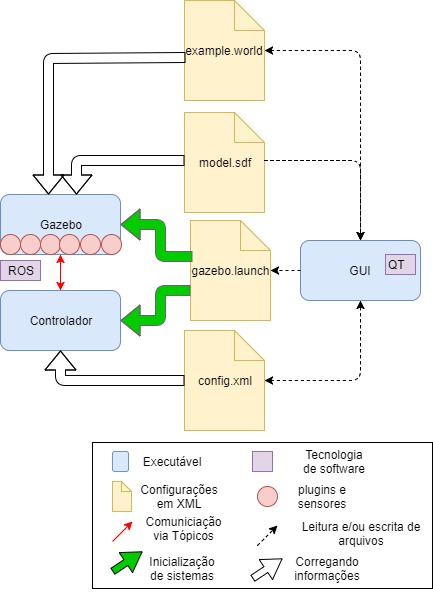
\includegraphics[width=0.65\textwidth]{figuras/estrutura.jpg}
	\caption{Esquemático do simulador}
	\label{Esquematico.jpg}
\end{figure}

O simulador Gazebo é o componente onde é executado o modelo do vant e, através de plugins e sensores, consegue-se obter e modificar dados durante execução do ambiente de simulação. Para sua configuração inicial, é necessário dois arquivos XML: ``model.sdf'' e ``example.world'' (pode-se escolher qualquer nome para este arquivo). Este descreve o cenário de simulação e aquele, o modelo de simulação.

O controlador, por sua vez, é o componente responsável por controlar o voo do vant. As configurações do controlador, tais como período de amostragem e tipo de estratégia de controle, são descritas em um arquivo denominado ``config.xml''.

Com o intuito de realizar comunicação entre Gazebo e Controlador e automatizar o seus respectivos processos de inicialização, utilizou-se características do ROS. A comunicação entre processos ocorre por meio de tópicos do ROS e a inicialização automática de processos, através de um arquivo XML denominado ``gazebo.launch''.

Por fim, com a finalidade de tornar amigável o processo de configuração da simulação, desenvolveu-se uma interface gráfica. A interface gráfica é um executável criado utilizando a API do QT, cuja função é ler e/ou editar os arquivos de configuração ``model.sdf'', ``gazebo.launch'' e ``config.xml'' (o sentido as setas na figura \ref{Esquematico.jpg} mostra o fluxo de informação entre o executável e tais arquivos).

Mais detalhes sobre tais elementos serão dados nos próximos capítulos do manual.


\chapter{Organização do projeto de software}

\hspace{1.5em}O diretório raíz do simulador é chamado \emph{ProVANT-Simulator}, no caso da versão estar no diretório destinado ao público, ou \emph{ProVANT-Simulator\_Developer}, para a versão em processo de desenvolvimento. Tal diretório está localizado, após a instalação, no diretório {\color{green}{\$HOME/catkin\_ws/src/}}. A figura \ref{fig:arvore_principal} ilustra a árvore de diretórios da estrutura do simulador ProVant. No diretório raíz, encontram-se duas pastas: \emph{doc} e \emph{source}: a pasta \emph{doc} contêm a documentação e os manuais de uso; e a pasta \emph{source} contêm o projeto de desenvolvimento da aplicação. 

\begin{figure}[htbp]
	\begin{forest}
		for tree={font=\sffamily, grow'=0,
			folder indent=.9em, folder icons,
			edge=densely dotted}
		[ProVANT-Simulator
		[ doc
		]
		[ source
		[build]
		[Database]
		[GUI]
		[Structure]
		]
		]
	\end{forest}
	\caption{Árvore dos diretórios principais do simulador ProVant.}
	\label{fig:arvore_principal}
\end{figure}

No primeiro nível da hierarquia do diretório raiz do simulador são encontrados os seguintes diretórios:

\begin{itemize}
	\itemsep0em
	\item \emph{build}: possui os arquivos binários  da interface gráfica. É gerado após a instalação completa do ambiente de simulação.
	\item \emph{Database}: possui arquivos de configuração de modelos, de cenários e da inicialização do ambiente de simulação.
	\item\emph{GUI}: possui o código fonte da interface gráfica.
	\item \emph{Structure}: possui o código fonte dos plugins e controlador; arquivos de dados gerados de simulação; e arquivos de descrição das mensagens de tópicos utilizadas para comunicação entre processos no ambiente de simulação. 
\end{itemize}



%\section{Diretório \emph{build}}
%\label{sec:d_build}
%
%\hspace{1.5em}O diretório \emph{build} contêm os arquivos binários, gerados pela compilação da interface gráfica.

\section{Diretório \emph{Database}}
\label{sec:d_database}

\hspace{1.5em}O diretório \emph{Database} é responsável por armazenar os cenários para o simulador, os modelos dos VANTs e arquivos de inicialização di ambiente de simulação. A estrutura interna do diretório  \emph{Database}, é ilustrado pela figura \ref{fig:arvore_database}.

\begin{tiny}
\begin{figure}[htbp]
\begin{forest}
	for tree={font=\sffamily, grow'=0,
    folder indent=.9em, folder icons,
    edge=densely dotted}
[Database
  [launch]
  [models]
  [worlds]
  [CMakeLists.txt, is file]
  [package.xml, is file]
]
\end{forest}
\caption{Árvore do diretório \emph{Database}.}
\label{fig:arvore_database}
\end{figure}
\end{tiny}

onde,

\begin{itemize}
	\itemsep0em
	\item \emph{launch}:  possui um arquivo denominado \emph{gazebo.launch}. Este é um arquivo escrito em \emph{XML} que se encarrega dos comandos de configuração do simulador, isto é, inicializa o ambiente do \emph{Gazebo} e executa o nó \emph{controller}.
	\item \emph{models}:  armazena modelos VANTs disponíveis.
	\item \emph{worlds}:  contem os arquivos de extensão \emph{world} correspondentes a descrição de cenários e configurações de simulação.
	\item \emph{CMakeLists.txt}: armazena informações para compilação de códigos fontes.
	\item \emph{package.xml}: armazena metadados do diretório, tais como nome e e enereço de e-mail do autor para contato. 
\end{itemize}

\section{Diretório \emph{GUI}}
\label{sec:d_GUI}

\hspace{1.5em}O diretório \emph{GUI} possui os arquivos \emph{.h} e \emph{.cpp} utilizados na implementação da interface gráfica.

\section{Diretório \emph{Structure}}
\label{sec:d_structure}

\hspace{1.5em}O diretório contém o código fonte de todos os componentes do ambiente de simulação, com exceção da interface gráfica. Além disso, é o local para armazenamento de arquivos de dados da simulação. A figura \ref{fig:arvore_structure} ilustra o diretório \emph{Structure}.

\begin{tiny}
\begin{figure}[H]
\begin{forest}
	for tree={font=\sffamily, grow'=0,
    folder indent=.9em, folder icons,
    edge=densely dotted}
  	[Structure
  		[Controller
  		]
  		[control\_strategies
  		]
  		[custom\_plugins
  		]
  		[Matlab
  		]
  		[simulator\_msgs
  		]
  	]
\end{forest}
\caption{Árvore do diretório \emph{Structure}.}
\label{fig:arvore_structure}
\end{figure}
\end{tiny}

\vspace{0.5em}
\noindent 

onde,

\begin{itemize}
	\itemsep0em
	\item \emph{Controller}: contem o código fonte do Controlador;
	\item \emph{control\_strategies}:contem o código fonte para diversas estratégias de controle;
	\item \emph{custom\_plugins}: possui o código fonte dos plugins.
	\item \emph{Matlab}: local onde se armazena arquivos com dados oriundos de simulações.
	\item \emph{simulator\_msgs}: contém arquivos de descrição de mensagens utilizadas para comunicação entre processos via tópicos do ROS. 
\end{itemize}
